\documentclass[a4paper, 12pt]{report}
%import package
%use xelatex to compile please !
\usepackage{amsmath}
\usepackage{paralist}
\usepackage{listings}
\usepackage[svgnames, table]{xcolor}
\usepackage{indentfirst}
\usepackage[CJKchecksingle, CJKnumber]{xeCJK}
%\usepackage{metalogo}
\usepackage[colorlinks,linkcolor=blue]{hyperref}
\usepackage[rm]{titlesec}% 改变章节标题格式
\usepackage{geometry}
\usepackage{booktabs}
\usepackage{graphicx}
\usepackage{enumitem}

%code highlight
\lstset{
    language = C,
    basicstyle = \ttfamily \small,
    flexiblecolumns = false,
    tabsize = 4,
    breaklines = true,
    basewidth = {0.5em, 0.45em},
    boxpos = t,
    backgroundcolor = \color[RGB]{245,245,244},
    keywordstyle = \bf\color{blue},
    %identifierstyle = \bf,
    commentstyle = \color[RGB]{0,139,0},
    numberstyle = \color[RGB]{0,192,192},
    stringstyle = \color[RGB]{128,0,0},
    rulesepcolor = \color[RGB]{102,102,102},
    frame = shadowbox,
    numbers = left,
    numbersep = 7pt
}

%setup Chinese & English fonts
%...
%\setmainfont[Mapping=tex-text]{Times New Roman}
\setmainfont[Mapping=tex-text]{Adobe Garamond Pro}
\setmonofont{Courier 10 Pitch}
\setCJKmainfont[BoldFont={Adobe Heiti Std}, ItalicFont={Adobe Kaiti Std}]{Adobe Song Std}
\setCJKsansfont{Adobe Heiti Std}
\setCJKmonofont{Adobe Fangsong Std}

\punctstyle{hangmobanjiao}
\parindent 2em
\linespread{1.2}
\setlist[description]{leftmargin=\parindent,labelindent=\parindent}

%编号层次
\setcounter{secnumdepth}{3} 
\setcounter{tocdepth}{3} 

%fix "no-break space" character error
%\DeclareUnicodeCharacter{00A0}{~}

%重命名
\renewcommand {\contentsname }{目\qquad 录}
\renewcommand {\listfigurename }{图\ 目\ 录}
\renewcommand {\listtablename }{表\ 目\ 录}
\renewcommand {\figurename }{图}
\renewcommand {\tablename }{表}
\renewcommand {\bibname }{参\ 考\ 文\ 献}
\renewcommand{\equationautorefname}{公式}
\renewcommand{\footnoteautorefname}{脚注}
\renewcommand{\itemautorefname}{项}
\renewcommand{\figureautorefname}{图}
\renewcommand{\tableautorefname}{表}
\renewcommand{\appendixautorefname}{附录}
\renewcommand{\theoremautorefname}{定理}
%\titleformat{\part}[display]{\centering\Huge}{\textbf{第~\thepart~部分}}{0.2cm}{}
\titleformat{\chapter}[block]{\centering\Huge\bfseries}{\textbf{第~\thechapter~章}}{1em}{}
\titleformat{\section}[block]{\LARGE\bfseries}{\textbf{\thesection}}{0.6em}{}
\titleformat{\subsection}[block]{\large\bfseries}{\textbf{\thesubsection}}{0.4em}{}
%自定义交叉引用
\newcommand{\secref[1]}{~\ref{#1}节}
\newcommand{\subsecref[1]}{~\ref{#1}小节}
%\newcommand{\tableref[1]}{表~\ref{#1}~}

%页面边距
\newgeometry{
    top=25mm, bottom=25mm, left=20mm, right=20mm,
    headsep=5mm, headheight=10mm, footskip=10mm,
}
\savegeometry{mgeometry}
\loadgeometry{mgeometry}

\renewcommand{\baselinestretch}{1.5}
\setlength{\parindent}{2em}
\setlength{\floatsep}{3pt plus 3pt minus 2pt}      % 图形之间或图形与正文之间的距离
\setlength{\abovecaptionskip}{10pt plus 1pt minus 1pt} % 图形中的图与标题之间的距离
\setlength{\belowcaptionskip}{3pt plus 1pt minus 2pt} % 表格中的表与标题之间的距离

%标题页
%Original author: Peter Wilson (herries.press@earthlink.net)
\newcommand*{\titleAT}{\begingroup % Create the command for including the title page in the document
\newlength{\drop} % Command for generating a specific amount of whitespace
\drop=0.1\textheight % Define the command as 10% of the total text height

\centering % Center all text
\rule{\textwidth}{1pt}\par % Thick horizontal line
\vspace{2pt}\vspace{-\baselineskip} % Whitespace between lines
\rule{\textwidth}{0.4pt}\par % Thin horizontal line

\vspace{\drop} % Whitespace between the top lines and title
\textcolor{Red}{ % Red font color
    {\Huge ARMv7支持}\\[0.5\baselineskip] % Title line 1
    {\Large OF}\\[0.75\baselineskip] % Title line 2
    {\Huge Barrelfish}} % Title line 3

\vspace{0.25\drop} % Whitespace between the title and short horizontal line
\rule{0.3\textwidth}{0.4pt}\par % Short horizontal line under the title
\vspace{\drop} % Whitespace between the thin horizontal line and the author name

{\large \textsc{陈逊,孙思杰}}\par % Author name

\vfill % Whitespace between the author name and publisher text
{\large \textcolor{Blue}{BUAALES}}\\[0.5\baselineskip] % Publisher logo
{\large \textsc{北京航空航天大学}}\par % Publisher

\vspace*{\drop} % Whitespace under the publisher text

\rule{\textwidth}{0.4pt}\par % Thin horizontal line
\vspace{2pt}\vspace{-\baselineskip} % Whitespace between lines
\rule{\textwidth}{1pt}\par % Thick horizontal line

\endgroup}

\begin{document}
    
    \pagestyle{empty} % Removes page numbers
    \titleAT % This command includes the title page
    %\maketitle
    %contents
    
    \tableofcontents
    %\listoffigures
    %\listoftables
	
	\chapter{施工进度}
    
    \begin{enumerate}
        \item 启动主路径:涉及内核初始化到init进程的全部过程,涉及文件:armv7 / boot.S,armv7 / boot\_driver.c,armv7 / bsp\_start.S,armv7 / cpu\_start.S,armv7 / init.c,armv7 / startup\_arch.c,arm / multiboot.c, armv7 / boot\_protocol.c。(未施工,孙思杰)
        \item 异常处理支持:armv7异常处理的实现,涉及文件有armv7 / set\_stack\_for\_mode.S,armv7 / exception.S,arm / exn.c。(\textcolor{red}{施工完毕})
        \item 板级支持:对一些ARMv7平台的板级支持,涉及文件有arm / jetsontk1\_uart.c,armv7 / plat\_a15mpcore.c,armv7 / plat\_id.c,armv7 / plat\_jetsontk1.c,armv7 / plat\_jetsontk1\_boot.c,armv7 / plat\_jetsontk1\_consts.c,armv7 / plat\_priv\_cbar.c。(\textcolor{red}{施工完毕})
        \item 中断处理支持:arm / gic.c,arm / irq.c。(\textcolor{red}{施工完毕})
        \item 时钟支持:arm / a15\_gt.c。(\textcolor{red}{施工完毕})
        \item Cache,TLB支持:kernel / include / arch / armv7 / cache.h。(\textcolor{red}{施工完毕})
        \item 虚存管理支持:关于MMU,页表等。涉及文件:cp15.h,armv7 / paging\_init.c,armv7 / paging.c。(\textcolor{red}{施工中})
        \item 系统调用支持:armv7 / syscall.c。(未施工)
        \item 线程调度支持:armv7 / disptch.c,arm / exec.c。(未施工)
        \item 串口输出支持:arm / kputchar.c。(\textcolor{red}{暂不施工})
        \item 调试支持:arm / gdb\_arch.c,arm / gdb\_arch.c,arm / debug.c。(\textcolor{red}{暂不施工})
    \end{enumerate}
    
    \chapter{概述}
    
    \section{概述}
    
    \textbf{TODO}
    
    \textbf{待施工}
    
    \section{ARMv7简述}
    
    ARMv7是ARM公司设计发布的一种精简指令集(RISC)架构,ARMv7-A是ARMv7体系结构中的A系列,主要面向于通用计算机,除此之外,还有面向实时的R系列和面向嵌入式低功耗低成本的M系列。ARMv7-A体系结构支持安全扩展(Security Extensions)和虚拟扩展(Virtualization Extensions),在现有的Barrelfish设计中并没有实现这些硬件特性,本文也没有对其进行实现,相关参数等保持缺省值。本文仅讨论ARMv7的ARMv7-A体系统结构,不适用于ARMv7-R和ARMv7-M型号的体系结构。
    
    \subsection{ARMv7的CPU模式}
    
    在ARMv7-A体系结构中,CPU被定义了9种工作模式,在任意时刻CPU只能处于其中一种状态。其中Monitor模式是为支持Security Extensions实现的,Hyp模式是为支持Virtualization Extensions实现的,在本文中不进行讨论。
    
    \begin{description}
        \item[用户模式(User mode)] 用户模式是唯一的一个非特权模式,一般用户级应用都运行在该模式下,在该模式下,应用无法直接访问被操作系统保护的系统资源。
        \item[系统模式(System mode)] 系统模式属于特权模式,和用户模式拥有同一组寄存器,不能通过异常进入该模式,该模式可以视作拥有特权的用户模式。
        \item[管理模式(Supervisor mode)] 管理模式是当系统调用发生时默认进入的模式,当计算机系统复位后也会自动进入该模式。ARM版本的Linux操作系统的内核态就是运行在这个模式下。
        \item[中止模式(Abort mode)] 当发生数据终止或者指令预取终止异常时进入该模式。
        \item[未定义模式(Undefined mode)] 当CPU检测到未定义的指令运行时进入该模式。
        \item[快速中断模式(FIQ mode)] 当FIQ中断发生时进入该模式,通常用于快速中断处理。
        \item[中断模式(IRQ mode)] 当IRQ中断发生时进入该模式,通常用于外部中断处理。
    \end{description}
    
    \subsection{ARMv7核心寄存器}
    
    在ARMv7-A体系结构中一共包含18个寄存器,部分寄存器在不同模式中有不同分组。在这些寄存器中有13个通用寄存器(R0-R12),其它分别为堆栈指针寄存器(SP),程序连接寄存器(LR),程序计数器(PC),当前程序状态寄存器(CPSR),保存程序状态寄存器(SPSR)。具体分组如\autoref{fig:armv7_reg}所示:
    
    \begin{figure}[htbp]
        \centering
        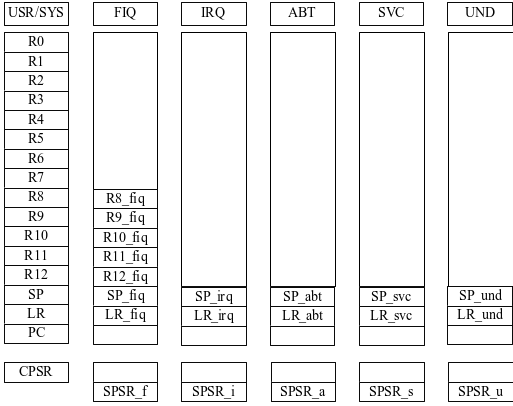
\includegraphics{./image/armv7_reg.png}
        \caption{ARMv7-A寄存器堆}
        \label{fig:armv7_reg}
    \end{figure}
    
    程序状态寄存器是ARM中用于记录程序状态的寄存器,分为当前程序状态寄存器(CPSR)和保存程序状态寄存器(SPSR)。CPSR记录当前程序运行状态信息,而SPSR用于进入异常后保存之前的CPSR值,用于恢复,每种异常CPU模式都有独立的SPSR分组。
    
    \begin{figure}[htbp]
        \centering
        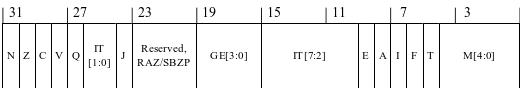
\includegraphics{./image/armv7_cpsr.jpg}
        \caption{CPSR位定义}
        \label{fig:armv7_cpsr}
    \end{figure}
    
    CPSR寄存器主要包含当前处理器模式,中断禁止位,条件标志及其他状态和控制位。CPSR组成如\autoref{fig:armv7_cpsr}所示。其主要位段介绍如下:
    
    \begin{description}
        \item[{M[4:0]}] 处理器模式,每一种模式有独立的编码。
        \item[F] 快中断屏蔽位。
        \item[I] 中断屏蔽位。
        \item[N] ALU负标志。
        \item[Z] ALU零标志。
        \item[C] ALU进位标志。
        \item[V] ALU溢出标志。
    \end{description}
    
    \chapter{板级支持}
    
    目前Barrelfish在ARMv7-A架构的支持上主要实现了对ARM Cotrex A9的PandaboardES,zynq7000和ARM Cortex A15的Vexpress的支持。我们实验室在此基础上实现了对Jetson-tk1开发板的支持。
    
    这一部分中,Cortex-A15共用的文件有armv7 / plat\_id.c, armv7 / plat\_a15mpcore.c, armv7 / plat\_priv\_cbar.c。plat\_id.c文件主要访问一些CP15协处理器的寄存器获取一些基本信息。plat\_priv\_cbar.c文件主要访问CP15的CBAR寄存器得到Private Peripheral Region的基址,初始化内核参数periphbase。下面主要介绍Jetson-tk1的相关实现。
    
    \section{串口驱动}
    
    在Jetson TK1 中设计实现了4个UART设备,分别编号为UART-A,UART-B,UART-C,UART-D。在设计和操作上,四个UART设备基本一致,均支持16450编程模式和16550编程模式。下面简单介绍一下UART的主要寄存器:

    \begin{description}
        \item[THR寄存器] 发送数据保持,用于存储发送数据,等待UART进行发送。
        \item[RBR寄存器] 接收数据缓冲,用于存储接收数据,等待CPU进行读取。
        \item[DLL寄存器] 波特率除数低位,用于设置波特率除数。
        \item[DLM寄存器] 波特率除数高位,用于设置波特率除数。
        \item[IER寄存器] 中断使能,其中IER[0]和IER[1]分别对应接收数据中断和THR寄存器空中断。
        \item[IIR寄存器] 中断识别,当中断发生时,用于标示中断的类型。
        \item[FCR寄存器] FIFO控制,用于控制FIFO。
        \item[LCR寄存器] 线控寄存器,用于设置数据位,停止位,奇偶校验和寄存器访问切换等。
        \item[MCR寄存器] 用于Modem控制。
        \item[LSR寄存器] 用于表示当前的通信状态。
        \item[MSR寄存器] 用于标示当前的Modem状态。
    \end{description}
    
    详细的寄存器介绍参见Jetson-tk1的技术手册,从技术手册中我们可以得到波特率除数的计算方法:
    \begin{lstlisting}[language=C]
    #define CONFING_SYS_NS16550_CLK         408000000
    #define CONFING_SYS_NS16550_BAUDRATE    115200
    static int calc_divisor(void)
    {
        const unsigned int mode_x_div = 16;
        return (CONFING_SYS_NS16550_CLK / mode_x_div
                / CONFING_SYS_NS16550_BAUDRATE );
    }
    \end{lstlisting}
    
    UART设备的时钟频率为408000000Hz,波特率为115200,波特率除数就等于时钟频率除以波特率再除以16。
    
    \subsection{内核实现}
    
    在文件kernel / arch / armv7 / plat\_jetsontk1\_consts.c中,定义了UART相关的常量,如UART的基址,大小,以及默认的UART编号。由于U-boot的相关设置,在这里我们直接设置选用UARTD(编号为3)。
    
    根据Jetson-tk1开发板技术手册,在devices / jetsontk1 / jetson\_uart.dev文件中实现对UART寄存器的描述。并在kernel / arch / arm / Jetsontk1\_uart.c中实现相关驱动。其主要函数如下:
    
    \textbf{jetson\_uart\_hw\_init函数}:该函数负责对UART的硬件进行初始化。参数uart给出进行初始化的对象。其主要流程如下:
    
    \begin{enumerate}
        \item 等待UART发送缓冲区为空。
        \item 置LSR寄存器DLAB位为1,以便写波特率除数寄存器。
        \item 清空波特率除数寄存器(包括低位寄存器和高位寄存器)。
        \item 置LSR寄存器DLAB位为0,以便写MCR寄存器。
        \item 设置MCR寄存器的DTR和RTS标志位。
        \item 设置FCR寄存器,禁用FIFOs和DMA,设置接收和发送的触发等级为0,并清除缓冲区。
        \item 设置IER,禁止所有中断。
        \item 置LSR寄存器DLAB位为1,设置波特率除数寄存器。
        \item 置LSR寄存器DLAB位为0。
        \item 设置IER寄存器,允许接收数据中断。
        \item 设置LSR寄存器控制位,8数据位,1停止位,无校验。
    \end{enumerate}
    
    \textbf{serial\_putchar函数}:该函数向串口输出一个字符,首先循环等待发送移位寄存器空,然后将数据写入发送移位寄存器中。
    
    \textbf{serial\_getchar函数}:该函数从串口读取一个字符,循环检查IIR寄存器,判断是否存在读数据中断等待,如果有从RBR寄存器中取出数据。
    
    \textbf{serial\_early\_init函数}:对jetson\_uart\_hw\_init函数的封装,用于CPU\_driver初期初始化串口,直接用串口的原始地址进行初始化。
    
    \textbf{jetson\_uart\_init函数}:与serial\_early\_init函数类似,不同的是:这个函数是将串口地址映射到内核设备地址空间后调用的,采用的是映射后的地址。其被kernel / arch / armv7 / plat\_jetsontk1.c中的serial\_init函数调用。
    
    \subsection{用户实现}
    
    目前Barrelfish用户层的串口支持在所有的平台上都采用系统调用的方式实现,具体代码见usr / drivers / serial文件夹\footnote{应用名为serial\_kernel,该目录下保留原有的驱动,如serial\_omap44xx等。},主要涉及的系统调用为sys\_print和sys\_getchar。注意需要对中断号进行相应的设置,如Jetson-tk1的UARTD中断号为122。
    
    \section{CPU电源管理}
    
    \subsection{Jetson-tk1 CPU加电}
    
    这里仅对启动APP核心进行描述,其他的CPU电源管理部分参见Jetson-tk1技术手册。启动第二个核的关键在于两点:一是,如何唤醒其他的处理器核心;二是,如何设置内核入口地址。
    
    关于第一点,Jetson TK1设计实现了被称作Flow Controller的设备来管理CPU的电源状态,在技术手册中给出了启动指定处理器核心的方法:
    
    \begin{enumerate}
        \item 设置FLOW\_CTLR\_CPUx\_CSR寄存器\footnote{x为CPU的编号}值为0x1。
        \item 设置FLOW\_CTLR\_HALT\_CPUx\_EVENTS寄存器\footnote{x为CPU的编号}值为0x48000000。
    \end{enumerate}

    关于第二点:关于第二点,在Jetson TK1 的技术手册中并没有给出具体的方法,只是指出处理器核心在复位后将从Reset vector寄存器指示的地址读取第一条指令且所有的处理器核心共用一个Reset vector寄存器,而并没给出Reset vector寄存器的设备地址。经过测试,最终确定Reset vector寄存器地址为0x6000f500。

    \subsection{Barrelfish实现}
    
    在kernel / arch / armv7 / plat\_jetsontk1\_boot.c文件中定义启动APP核心的关键函数plat\_advance\_aps,该函数初始化Flow Controller设备,设置启动地址,并依次唤醒3个APP核心。
    
    \chapter{异常处理支持}
	
	\section{ARMv7异常处理}
    
    \subsection{异常种类和向量表}
    
    在ARMv7-A体系结构中,主要的异常有7种,分别是快速中断请求,中断请求,SWI,复位,数据中止,指令预取中止和未定义指令。每一种异常都有对应的CPU模式。其对应关系如\autoref{table:exceptions}所示。
    
    \begin{table}[htbp]
    \centering
    \caption{ARMv7异常模式}
    \label{table:exceptions}
    \begin{tabular}{llccl}
        \toprule
        异常 & CPU模式 & 偏移 & 优先级 & 备注 \\
        \midrule
        Reset & Supervisor & +0x00 & 1 & 系统复位异常 \\
        Undefined instrucion & Undefined & +0x04 & 6 & 未定义指令异常 \\
        Software Interrupt(SWI) & Supervisor & +0x08 & 6 & 软件中断异常 \\
        Prefetch Abort & Abort & +0x0c & 5 & 指令预取中止异常 \\
        Data Abort & Abort & +0x10 & 2 & 数据中止异常 \\
        IRQ & IRQ & +0x18 & 4 & 中断请求异常 \\
        FIQ & FIQ & +0x1c & 3 & 快中断请求异常 \\
        \bottomrule
    \end{tabular}
    \end{table}
    
    \subsection{异常处理过程}
    
    与X86处理器类似,ARMv7-A也采用异常向量表的方式进行异常处理。但需要注意的是,在X86处理器中,异常向量表中的每一项包含的是对应的处理函数的入口地址,而在ARM处理器中,异常向量表的每一项包含的是跳转到对应处理函数的跳转指令。
    
    在ARMv7-A中,异常向量表被规定了固定的地址1,该地址具体由CP15中的SCTLR寄存器的V位确定,当SCTLR.V等于0时,异常向量表位于0x00000000地址处,当SCTLR.V等于1时,异常向量表位于0xFFFF0000处。
    
    当异常发生时,CPU会自动执行如下过程:首先,将CPSR保存到该异常的SPSR寄存器中。然后,将PC保存到该异常模式的LR寄存器中。接着,将CPSR中的模式位设置为相应的异常模式。最后,根据该异常在向量表中的偏移,读取对应跳转指令执行。在此之后,由操作系统接管控制,进行相应的异常处理。每种异常对应的偏移如\autoref{table:exceptions}所示。
	
	\section{Barrelfish实现}
    
    在Barrelfish中,主要实现了对数据中止,指令预取中止,快速中断请求,中断请求,未定义和SWI异常的处理接口,没有实现复位异常的处理接口。
    
    \subsection{异常初始化}
    
    在Kernel启动的过程中,会对异常进行初始化,相关调用在kernel / arch / armv7 / init.c中可以看到,其主要的工作有两点:初始化CPU各个异常模式的堆栈指针(SP);初始化异常向量表页表映射。
    
    \textbf{set\_stack\_for\_mode函数}:为指定的CPU异常模式设置堆栈指针,相关文件为kernel / arch / armv7 / set\_stack\_for\_mode.S,代码很简单不再赘述。
    
    \textbf{paging\_map\_vectors函数}:初始化异常向量表的页表映射,在BSP核启动是被调用(\textcolor{red}{存疑}),该函数定义在kernel / arch / armv7 / paging.c中。
    
    函数的基本过程如下:确定异常向量表的物理地址,及kernel / arch / armv7 / exceptions.S文件中的exception\_vectors函数地址;设置二级页表项;设置一级页表项;废弃对应页表的Cache行。
    
    \subsection{异常向量表}
    
    在异常处理中,比较关键的问题是如何设置好各种异常对应的处理函数,即如何初始化异常向量表。在第2章中提到过,不同于X86平台,ARM规定异常向量表中的每一项应该是完整的指令,由于指令的编码限制,无法实现向量表跳转到4GB空间的任意地址。文献[15]中提出一种方法解决了上述限制,使得异常处理接口可以位于任意地址。具体方法描述如下\textcolor{red}{(废弃)}:在异常向量表之后的固定偏移处设置一个跳转表,跳转表的每一项包含对应的异常处理接口的入口地址;在异常向量表中,每一项设置为一条LDR指令,这条指令能将对应的跳转表项中地址加载到PC寄存器中,从而实现跳转。\textcolor{blue}{新的实现方法为}:异常向量表不能实现长跳转,但可以实现短跳转,异常向量表中的每一条跳转指令被设置为跳转的同一4k页面的对应汇编处理接口,由其实现跳转到对应的C编写的二级异常处理接口。
    
    \subsection{异常处理接口}
    
    关于异常处理接口,通常分为两级,第一级由汇编代码编写,主要完成现场的保存,屏蔽中断,进入内核态,调用第二级处理接口;第二级由C语言编写,完成实际的异常处理,下面分别进行介绍。
    
    以irq异常为例介绍一级异常处理接口的实现,其他类型的异常类似。处理irq异常的一级处理接口函数为irq\_handler,其主要流程为:判断是内核irq异常还是用户irq异常;如果是内核irq异常,这不用进行现场保存(原因为内核irq异常是发生在wfi循环中,不用关心寄存器状态),调用enter\_sys宏切换到SYS模式,跳转到第二级异常处理接口执行;如果是用户irq异常,首先判断当前Dispatcher的状态为disable还是enable,然后根据Dispatcher状态保存寄存器现场,进入SYS模式,跳转到第二级异常处理接口执行。
    
    下面分别介绍主要的第二级异常处理接口,主要涉及的文件有kernel / arch / armv7 / syscall.c和。
    
    \textbf{sys\_syscall函数}:SWI异常的处理接口,响应用户的系统调用请求,接口定义如下:
    
    \begin{lstlisting}
    void sys_syscall(arch_registers_state_t* context,
            uint32_t disabled,
            struct dispatcher_shared_arm *disp)
    \end{lstlisting}
    
    参数context指出保存的寄存器现场,disable指出当前的Dispatcher状态,disp指出内核中Dispatcher的指针。此函数通过resume函数恢复调用这的现场,以此返回到调用函数。
    
    函数的主要流程如下:检查Dispatcher状态,解析系统调用参数;判断系统调用类型,调用相应的处理接口;将处理接口的返回结构和错误代码\footnote{不一定表征出现错误,当值为SYS\_ERR\_OK表示结果正确。}封装成sysret结构体,写入寄存器现场,调用resume恢复调用者现场。
    
    \textbf{handle\_user\_undef函数}:未定义指令异常处理接口,主要处理流程如下:检查Dispatcher状态;跳转到Barrelfish库的用户层dispatcher\_trap接口执行,并设置相应的参数,屏蔽快中断切换到用户模式;调用resume完成跳转。
    
    \textbf{handle\_user\_page\_fault函数}:用户数据或预取指令中止异常处理接口,处理用户程序出现的页面错误。其主要流程如下:检查Dispatcher状态;根据Dispatcher状态设置相应的用户层接口(Barrelfish库):disable对应dispatcher\_pagefault\_disabled,并将页面错误计数加1,enable对应dispatcher\_pagefault;如果disable状态下发生页面错误超过3次,则将该Dispatcher移出调度队列,调度其他Dispatcher,如果是enable状态调用resume切断到用户层页面处理接口。
    
    \textbf{fatal\_kernel\_fault函数}:内核中不应该发生未定义指令,数据中止,指令预取中止,如果出现将是致命的,这个函数只负责将错误相关的内核参数和寄存器内容打印出来,以供调试。
    
    \textbf{handle\_irq\_kernel函数}:内核中一般来说不应该出现中断的,除了内核在wait\_for\_interrupt函数中等待(sleep)。检查waiting\_for\_interrupt变量确定内核是否在等待中断,如果是交由irq\_handler函数处理,如果不是说明出现致命错误,调用fatal\_kernel\_fault函数。
    
    \textbf{irq\_handler函数}:响应快中断和中断异常,在Barrelfish暂时不对两这进行区分。主要流程如下:检查Dispatcher状态;从中断控制器获取active的中断号;如果是时钟中断,进行Dispatcher调度,反之通知用户中断处理接口接手。
    
    \subsection{多核异常处理}
    
    Barrelfish的多内核模型决定了不同的处理器核心上的内核应该有自己独立异常向量表,在多内核模式下,各个内核的异常向量表的映射关系如\autoref{table:exception_vector}所示。从表中可以看出,Barrelfish为一个异常向量表分配的内存空间为4KB,所以异常向量表所在区域应该采用二级页表的方式映射。
    
    \textcolor{red}{在新版本中,由于CPU driver共用一个页表,导致异常向量表映射到同一个地址,所有内核共用同一段异常处理接口代码。这与Barrelfish核心思想相悖,待讨论。}
    
    \begin{table}[htbp]
        \centering
        \caption{多核异常向量表映射}
        \label{table:exception_vector}
        \begin{tabular}{ccc}
            \toprule
            处理器核心 & 异常向量表虚拟地址 & 异常向量表物理地址  \\
            \midrule
            Core 0 & 0xFFFF0000 & 0x800F0000  \\
            Core 1 & 0xFFFF0000 & 0x800F1000  \\
            Core 2 & 0xFFFF0000 & 0x800F2000  \\
            Core 3 & 0xFFFF0000 & 0x800F3000  \\
            \bottomrule
        \end{tabular}
    \end{table}
    
    \chapter{中断处理支持}
    
    \section{ARMv7中断处理}
    
    \subsection{概述}
    
    ARM Cortex A15 处理器采用的是 ARM 中断控制体系结构第二版,主要功能有:中断屏蔽,中断优先级设置,中断分发,中断状态跟踪,软件中断的生成等。在 ARM 中,中断控制器(GIC)被分成了两个部分,一个被称为 Distributor,另一个称为 CPU interface。Distributor 主要功能是接收所有中断,判断优先级,并将优先级最高的中断转发给对应的 CPU interface 。CPU interface 主要功能是接收 Distributor 转发的中断,识别并裁决中断,维护中断状态机,转发优先级适宜的中断给目标处理器核心,每一个处理器核心都有自己单独的CPU interface。

    在ARM中,中断源被分为三种,一是软件生成中断\footnote{Software Generated Interrupts,缩写为 SGIs。},二是专用外设中断\footnote{Private Peripheral Interrupts,缩写为 PPIs。},三是共享外设中断\footnote{Shared Peripheral Interrupts,缩写为SPIs。}。一般情况下,软件生成中断用于处理器核间通信,也就是所谓的核间中断\footnote{Inter-Processor Interrupt,缩写为IPI。},专用外设中断主要用于核心专用外设如专用时钟的通信,共享外设中断用于处理器共享设备诸如键盘,串口等的通信。软件生成中断的中断号范围为ID0-ID15,专用外设中断的中断号范围为ID16-ID31,共享外设中断使用的中断号范围为ID32-ID1019。
    
    这一部分主要参考了ARMv7-技术手册和ARM中断控制技术手册,如果有不解或不详细的地方请查证原文。
    
    \subsection{Distributor}
    
    Distributor管理全局的中断转发,每个中断的允许或禁止,中断的分组等,是GIC的最外层接口。Distributor中有一系列的寄存器用于管理中断,下面就比较重要的寄存器进行分析。

    GICD\_CTLR寄存器:是Distributor的控制寄存器,主要用于允许或禁止全局中断的转发。该寄存器的EnableGrp0位和EnableGrp1位分别控制第0组中断和第1组中断到CPU interface的转发,控制位为1时,允许对应分组的转发。
    
    GICD\_IGROUPRn寄存器集:该寄存器集控制每一个中断所属的分组。每一个寄存器共有32位,可以设置32个中断的分组,每一位用0表示对应中断为第0组,用1表示对应中断为第1组。
    
    GICD\_ISENABLERn寄存器集:该寄存器集控制指定中断到CPU interface的转发。每一个寄存器有32位,分别对应32个中断的使能,当某中断在对应寄存器中的对应位为1时,Distributor允许该中断到CPU interface的转发。
    
    GICD\_IPRIORITYRn寄存器集:该寄存器集控制指定中断的优先级。每一个中断的优先级占8位,所以每个寄存器对应4个中断的优先级设置。值得注意的是,中断优先级并不一定使用全部的8位,视具体的实现而定。
    
    GICD\_ITARGETSRn寄存器集:该寄存器集控制指定中断的目标处理器。每一个中断需要8位,所以每个寄存器对应4个中断的目标处理器设置。对于每一个中断而言,8位对应着8个CPU interface,8位中的某一位置1,则允许该中断转发给对应的CPU interface。
    
    GICD\_ICFGRn寄存器集:该寄存器集控制指定中断的触发方式,电平触发或边缘触发。每个中断设置需要占2位,即每个寄存器对应16个中断的触发方式设置。对于每一个中断而言,具体规则如下:
    
    \begin{enumerate}
        \item 如果中断为SGI中断,则该中断对应位只读,值恒为0b10,边缘触发。
        \item 如果中断为PPI中断,则该中断对应位只读,值恒为0b01,电平触发。
        \item 如果中断为SPI中断,则该中断对应位可读写,如果值为0b01,为高电平触发,如果值为0b11,为边缘触发。
    \end{enumerate}
    
    \subsection{CPU interface}
    
    CPU interface是处理器核心的中断接口,处理发送到对应处理器的中断,维护每个中断的状态机,转发优先级适宜的中断到对应的处理器核心,下面就比较重要的寄存器进行分析。

    GICC\_CTLR寄存器:CPU interface控制寄存器,主要功能是控制中断到对应处理器核心的转发。
    
    GICC\_PMR寄存器:CPU interface中断屏蔽寄存器,主要功能是屏蔽低于指定优先级的中断转发。通过写该寄存器的低8位,可以设置屏蔽优先级。
    
    GICC\_IAR寄存器:CPU interface中断识别寄存器,主要功能是提供当前激活的中断号,如果该中断为SGI中断,并提供发出该请求的处理器ID。
    
    GICC\_EOIR寄存器:CPU interface中断结束寄存器,在中断处理结束后,操作系统通过将中断号写入GICC\_EOIR寄存器,向中断控制器报告中断处理完毕。
    
    \section{Barrelfish实现}
    
    一般操作系统在中断方面的处理大概分为两个部分:中断控制器的驱动\footnote{主要涉及的文件为kernel / arm / gic.c}和用户中断的支持\footnote{主要涉及的文件为kernel / arm / irq.c}。下面从上述两个方面分别阐述Barrelfish对ARMv7的支持。
    
    \subsection{中断控制器驱动}
    
    中断控制器,简称GIC,是硬件提供给操作系统的中断控制接口,表现为一系列的可读写寄存器。在Barrelfish中设备的寄存器I/O接口(C语言)由Mackerel描述文件编译给出,中断控制器的Mackerel文件位于devices / pl130\_gic.dev,其主要描述了各个寄存器的偏移,位段定义和一些注释性的描述。关于Mackerel语言的相关信息参见Barrelfish官方相关文档。
    
    在给出了中断控制器的寄存器I/O接口后,就需要实现用于支持用户中断处理的驱动程序。在Barrelfish中定义和实现了如下的接口:
    
    \textbf{中断控制器初始化}:这个函数完成对中断控制器的初始化工作,一般在内核初始化阶段(详见kernel / arch / armv7 / init.c文件)调用执行。其定义如下:
    
    \begin{lstlisting}[language=C]
    void gic_init(void)
    \end{lstlisting}
    可以看出这个函数不需要参数也没有返回值,考虑一下为什么返回一个表征成功与否的返回值呢?从函数中可以分析可到ARMv7中断控制器的初始化步骤:
    \begin{enumerate}
        \item 映射设备地址到内核的虚拟地址空间,这里需要注意的是三个地址:ARM PERIPHBASE,Distributor偏移,CPU interface偏移,前者由硬件厂商确定,后两者由ARMv7中断手册给出\footnote{在Jetson-tk1开发板中PERIPHBASE为0x5400:0000,ARMv7中Distributor偏移为0x1000,CPU interface偏移为0x2000}。
        \item 读取ICDICTR寄存器,获得Interrupt lines和cpu\_number信息。
        \item 设置CPU interface优先级掩码为0xff,接受所有中断。
        \item 设置binary point为2,其作用参见ARMv7中断手册。
        \item 设置ICCICR寄存器,允许中断转发到处理器。
        \item 设置ICDDCR寄存器,允许Distributor转发中断给CPU interface。
    \end{enumerate}
    
    \textbf{获取激活中断}:当一个中断处于激活(Active)状态时,中断控制器将在ICCIAR寄存器中给出处于Active状态的中断源编号。其函数定义如下:
    
    \begin{lstlisting}[language=C]
    uint32_t gic_get_active_irq (void)
    \end{lstlisting}
    该函数从ICCIAR寄存器中读取出Active的中断编号,然后返回该值。
    
    \textbf{生成软中断}:中断控制器的ICDSGIR寄存器提供了生成软中断的功能,向该寄存器写入目标cpu和中断编号即可生成一个软中断。该函数定义如下:
    
    \begin{lstlisting}
    void gic_raise_softirq(uint8_t cpumask, uint8_t irq)
    \end{lstlisting}
    参数cpumask给出目标cpu的编号,irq给出软中断的编号,SGI一共16个,所以定义为uint8\_t。
    
    \textbf{中断应答}:当内核进行中断处理时,用于通知中断控制器,操作系统已经对中断做出了相应。该函数定义如下:
    
    \begin{lstlisting}[language=C]
    void gic_ack_irq(uint32_t irq)
    \end{lstlisting}
    参数irq指出操作系统应答的中断号。
    
    \textbf{CPU interface中断转发使能}:该函数使能CPU interface到Processor的转发。
    
    \textbf{指定中断的使能}:该函数中断控制器驱动的关键函数之一,根据给出的参数使能一个指定中断的触发。函数定义下:
    
    \begin{lstlisting}[language=C]
    void gic_enable_interrupt(uint32_t int_id, uint8_t cpu_targets, uint16_t prio, bool edge_triggered, bool one_to_n)
    \end{lstlisting}
    参数int\_id给出指定中断的中断号\footnote{一般可以通过硬件厂商的技术手册查询得到},参数cpu\_targets给出目标cpu,prio指定中断优先级,edge\_trriggered确定是边缘触发还是电平触发,one\_to\_n确定是一对一还是一对多的中断。函数的基本流程如下:
    
    \begin{enumerate}
        \item 一般性检查和中断类型确定。
        \item 设置ICDISER寄存器\textbf{集}中对应的中断使能位,中断号除以32确定寄存器集中的对应寄存器编号,余数确定在该寄存器中的位偏移,后面的寄存器\textbf{集}类似。
        \item 通过ICDIPR寄存器\textbf{集}设置该中断的中断优先级。
        \item 如果是SPI类型的中断源,通过ICDIPTR寄存器\textbf{集}设置目标cpu。
        \item 通过ICDICR寄存器\textbf{集}设置触发方式和分发方式。
    \end{enumerate}
    
    \subsection{用户中断支持}
    
    Barrelfish内核通过IRQ dispatch table这样一个数组管理用户中断分发,该数组每个元素都是一个Capability Table Entry结构体,用于存储负责处理该中断的Dispatcher的Endpoint。Barrelfish支持32个CPU内部中断(PPI和SGI)和128个SPI中断,所以数组共160个元素。
    
    当用户程序向内核注册中断时,内核设置好irq\_dispatch数组并在中断控制器中使能该中断。当该中断被触发时,系统进入中断异常,内核处理时钟中断,其他中断会通知用户层Barrelfish的库代码进行处理\footnote{代码位于lib/barrelfish/文件夹中,尚未分析}。\textcolor{red}{注意内核对用户中断的支持仅限于中断的分发。}
    主要函数如下:
    
    \textbf{irq\_table\_set函数}:该函数对用户中断进行注册,即设置对应的用于IDC通信的Endpoint Capability并硬件中断使能。函数定义如下:
    
    \begin{lstlisting}[language=C]
    errval_t irq_table_set(unsigned int nidt, capaddr_t endpoint)
    \end{lstlisting}
    参数nidt指出中断源的编号,参数endpoint指出Endpoint的capability地址,返回值给出错误Code。该函数首先根据endpoint给出的地址从当前Dispatcher的Cspace中取出对应的Capability Table Entry,拷贝到irq\_dispath数组中,然后在中断控制器中使能该中断。
    
    \textbf{irq\_table\_delete函数}:该函数注销用户中断,即将对应的irq\_idspatch数组项删除。
    
    \textbf{irq\_table\_notify\_domains函数}:\textcolor{red}{TODO}。
    
    \textbf{send\_user\_interrupt函数}:该函数通知用户Dispatcher对中断进行响应,并立刻调度该Dispatcher执行。其函数定义如下:
    
   \begin{lstlisting}[language=C]
   void send_user_interrupt(int irq)
   \end{lstlisting}
    参数irq给出中断源编号,该函数从irq\_dispatch数组中取出Endpoint的Capability,调用lmp\_deliver\_notification通知Dispatcher中断的发生,之后立即调度该Dispatcher运行。

    \chapter{时钟支持}
    
    \section{ARMv7时钟}
    
    \label{section:armv7Timer}
    
    \subsection{概述}
    
    在ARMv7-A体系结构中,ARM设计了一个通用的时间子系统,被称作Generic Timer。该时间子系统主要由两部分组成,一个是位于处理器外部通过系统时钟总线相连的System counter,另一个是与处理器核心直接相连的Timer,在对称多处理机上,一般有一个System counter和多个Timer。
    
    \subsection{System Counter}
    
    System Counter是一个全局的计数器,其从机器加电开始,以一定的频率做自增运算,提供一个全局统一的系统时间。除了基本的计时功能,System Counter还具有事件流(event stream)的功能,用于产生周期性的事件。下面就比较重要的寄存器进行介绍。

    \textbf{CNTFRQ寄存器}:计数器频率寄存器,主要功能是设置System Counter的频率。
    
    \textbf{CNTKCTL寄存器}:时钟控制寄存器,主要功能是设置时钟访问权限和事件流,需要注意的是,控制寄存器并没有提供重置System Counter的功能。
    
    \subsection{Timers}
    
    每一个处理器核心都有多个专用的Timer(定时器),用于产生时钟中断。在时间子系统中,System Counter的值会被广播到各个Timer中,Timer根据System Counter的值来判断时钟已经达到设定值,当时钟到达设定值,Timer就会产生时钟中断。根据是否支持安全扩展和虚拟扩展,一个处理器核心上Timer的个数不同,本文中从略。本文中所涉及的Timer均为通用的PL1 Physical Timer,其中断号为29。
    
    其主要寄存器如下:

    \textbf{CNTP\_CTL寄存器}:PL1物理时钟控制寄存器,主要功能是标示事件状态,时钟使能,中断屏蔽。具体位段解释如下:
    
    \begin{description}
        \item[ENABLE] 当该位为1时,使能该Timer。
        \item[IMASK] 当该位为1时,屏蔽该Timer的输出信号,即不产生时钟中断。
        \item[ISTATUS] 当该位为1时,表明时钟条件已经达到。
    \end{description}
    
    \textbf{CNTP\_TVAL寄存器}:该寄存器设置一个自减计数器的值,每当System counter加一,该计数器值减一,当该计数器的值为0时,产生时钟中断。
    
    \textbf{CNTP\_CVAL寄存器}:该寄存器设置一个自加计数器的值,当System counter的值达到该值时,产生时钟中断。
    
    \section{Barrelfish实现}
    
    Barrelfish采用了ARM Cortex-A15的Generic Timer实现了其时钟子系统,对于每个CPU核心的4个定时器(Timer)来说,Barrelfish只利用了其PL1 Physical Timer。其中System Counter模块为整个系统提供全局统一的时钟,而每个Timer为每一个CPU driver提供定时器,并产生时钟中断,从而为Barrelfish的进程分时调度提供支持。
    
    \subsection{时钟I/O接口}
    
    ARM Cortex-A15 Generic Timer寄存器全部为CP15协处理器寄存器。Barrelfish在kernel / include / arch / armv7 / a15\_gt.h文件中实现了Timer相关寄存器的I/O接口。简要描述由\autoref{table:timer_reg}给出,详细的寄存器定义见\secref[section:armv7Timer]和ARMv7技术手册。
    
    \begin{table}[htbp]
        \centering
        \caption{时钟I/O接口}
        \label{table:timer_reg}
        \begin{tabular}{lll}
            \toprule
            函数名 & 相关寄存器 & 注解 \\
            \midrule
            a15\_gt\_frequency & CNTFRQ & 读取System Counter的频率,单位Hz \\
            a15\_gt\_set\_cntfrq & CNTFRQ & 设置System Counter的频率,单位Hz \\
            a15\_gt\_counter & CNTPCT & 读取System Counter的值 \\
            a15\_gt\_timeout & CNTP\_CVAL & 读取定时器的超时值 \\
            a15\_gt\_set\_control & CNTP\_CTL & 设置Physical Timer的控制寄存器 \\
            a15\_gt\_set\_comparator & CNTP\_CVAL & 设置Physical Timer的CompareValue \\
            a15\_gt\_mask\_interrupt & CNTP\_CTL & 屏蔽Physical Timer的中断 \\
            \bottomrule
        \end{tabular}
    \end{table} 
    
    \textbf{a15\_gt\_set\_comparator函数}:该函数设置定时器的CompareValue,一般该值比System Counter值大,当System Counter的值达到CompareVaule时,并且定时器被使能,中断未被屏蔽,定时器就会产生时钟中断。该函数首先设置CNTP\_CVAL的值为CompareValue,然后设置CNTP\_CTL寄存器使能定时器并\textbf{清除中断屏蔽位}。
    
    \textbf{a15\_gt\_init函数}:该函数主要对三个控制寄存器(CNTKCTL,CNTP\_CTL,CNTV\_CTL)进行初始化,函数定义在kernel / arch / armv7 / a15\_gt.c文件中,函数流程如下:设置CNTKCTL寄存器使能用户空间(PL0)访问Physical Timer,设置CNTV\_CTL寄存器禁用Virutal Timer,设置CNTP\_CTL寄存器使能Physical Timer并屏蔽其中断信号。
    
    \subsection{时钟驱动}
    
    Barrelfish中时钟驱动的主要作用是产生时间片,应答时钟中断,提供系统时间戳。相关代码可以在kernel / arch / armv7 / plat\_a15mpcore.c文件中可以看到,主要函数如下:
    
    \textbf{timers\_init函数}:该函数初始化时钟,并在中断控制器中允许时钟中断,并设置第一次时钟超时。函数定义如下:
    \begin{lstlisting}[language=C]
    void timers_init(int timeslice)
    \end{lstlisting}
    参数tiemslice给出了CPU driver的时间片长度,单位为ms。该函数首先设置System Counter频率,初始化时钟,然后在中断控制器中允许时钟中断,最后设置第一次超时。
    
    \textbf{timestamp\_read函数}:该函数返回当前System Counter值。
    
    \textbf{timestamp\_freq函数}:该函数返回System Counter的频率。
    
    \textbf{timer\_interrupt函数}:该函数首先调用gic\_ack\_irq函数应答中断控制器,并屏蔽Timer的中断,最后设置下一次超时。
    
    \textbf{systime\_now函数}:类似与timestamp\_read函数。
    
    \textbf{systime\_set\_timeout函数}:根据参数设置下一次发生时钟中断的超时值。
    
    \chapter{虚存管理}
    
    \section{ARMv7虚存管理}
    
    ARMv7-A包含一个内存管理单元(MMU)和相应的TLB和Cache,用于管理和映射虚拟内存。在ARMv7-A体系结构中,采用32位地址,共4GB地址空间。
    
    \subsection{MMU控制}
    
    MMU主要用于自动的地址映射,其能通过查询操作系统设置的页表,将虚拟地址转换实际的物理地址。

    ARMv7-A中,MMU通过CP15协处理器中的SCTLR寄存器进行设置,SCTLR寄存器的第一位就是MMU的使能位,将其置1就能启用MMU,示例代码如下:
    
    %% lstlisting 不支持ARM GNU ASM高亮......
    \begin{lstlisting}
    ldr r1, =0x1
    mrc p15, 0, r0, c1, c0, 0  // 读取SCTLR寄存器
    orr r0, r0, r1 //最低位置位
    mcr p15, 0, r0, c1, c0, 0	// 使能MMU
    \end{lstlisting}
    
    \subsection{TLB控制}
    
    与MMU相同,TLB同样通过CP15协处理器进行设置,这里主要涉及到TLB的清除操作,根据具体实现的不同,指令TLB和数据TLB可以统一或分离。如果TLB为统一的,直接清除快表即可,否则,需要分别清除指令TLB和数据TLB。

    示例代码如下:
    
    \begin{lstlisting}
    mcr p15, 0, r0, c8, c5, 0 // ITLBIALL,清除指令快表项
    mcr p15, 0, r0, c8, c6, 0 // DTLBIALL,清除数据快表项
    mcr p15, 0, r0, c8, c7, 0 // TLBIALL,清除统一快表项
    \end{lstlisting}
    
    \subsection{页表}
    
    在ARMv7-A中,支持两级页表,第一级页表将4GB的地址空间分为大小为1MB的段或者大小为16GB的超级段,二级页表将每一个一级页表段分为大小为4KB的页或者大小为16KB的大页,除此之外ARMv7-A还将页表项格式分为短描述符和长描述符两种,短描述符用于一般的虚存管理,而长描述符是用于支持物理地址扩展(Large Physical Address Extension)。CP15协处理器中的TTBCR寄存器的EAE位决定是采用短描述符还是长描述符,本文中采用短描述符格式。

    为了实现快速的虚拟地址空间切换,ARMv7-A将4GB地址空间分为两个部分,高地址区域一般用于映射操作系统内核地址空间和设备IO地址空间,低地址区域一般用于映射用户地址空间。具体的空间大小划分由CP15协处理器中的TTBCR寄存器的N位段决定,其编码如\autoref{table:pagetable}所示,比如当TTBCR.N为0b001时,内存区域被分为大小均为2GB的两个区域。
    
    \begin{table}[htbp]
        \centering
        \caption{内存划分规则}
        \label{table:pagetable}
        \begin{tabular}{ccc}
            \toprule
            TTBCR.N & TTBR0管理的内存区域 & TTBR1管理的内存区域  \\
            \midrule
            0b000 & 0x0 – 0xFFFFFFFF & -  \\
            0b001 & 0x0 – 0x7FFFFFFF & 0x80000000 – 0xFFFFFFFF  \\
            0b010 & 0x0 – 0x3FFFFFFF & 0x40000000 – 0xFFFFFFFF  \\
            0b011 & 0x0 – 0x1FFFFFFF & 0x20000000 – 0xFFFFFFFF  \\
            0b100 & 0x0 – 0x0FFFFFFF & 0x10000000 – 0xFFFFFFFF  \\
            0b101 & 0x0 – 0x07FFFFFF & 0x08000000 – 0xFFFFFFFF  \\
            0b110 & 0x0 – 0x03FFFFFF & 0x04000000 – 0xFFFFFFFF  \\
            0b111 & 0x0 – 0x01FFFFFF & 0x02000000 – 0xFFFFFFFF  \\
            \bottomrule
        \end{tabular}
    \end{table}
    
    ARM将内存分为两个区域后,为了实现上下文的快速切换,自然需要两个页表。一个是内核页表,在进程切换时不用切换,另一个是用户进程页表,在进程切换时,需要更改。在ARMv7-A体系结构中,使用两个寄存器来存储上述两个页表的基址,这两个寄存器分别是TTBR0和TTBR1,通过CP15协处理器进行操作。在切换页表时,只需要将新页表的物理地址写入对应的TTBR寄存器即可。

    需要特别注意的是,在切换页表之后为了使其立即生效,应当清除Cache和TLB,否则,可能读取到错误的指令或者数据。
    
    \section{Barrelfish实现}
    
    在内核中,Barrelfish在ARM上实现的虚存映射比较简单。Barrelfish将4GB虚拟地址空间分为大小均为2GB的区域,低2GB为用户地址空间,高2GB为内核地址空间。在页表的实现方面,除了异常向量表所在区域采用二级页表映射外,其他均采用一级页表,将物理内存划分为大小为1MB的段,并且采用一一对应的映射方式。
    
    主要的内存映射如\autoref{fig:mem_mapping}所示。
    
    \begin{figure}[htbp]
        \centering
        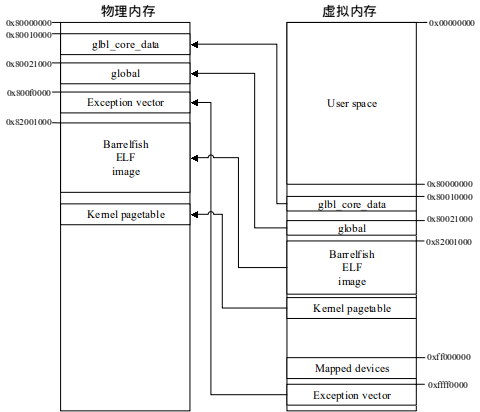
\includegraphics{./image/mem_mapping.png}
        \caption{Kernel内存映射}
        \label{fig:mem_mapping}
    \end{figure}
    
    用户进程的页表由用户层Barrelfish库完成。
    
    \subsection{Cache和TLB支持}
    
    Barrelfish根据ARMv7-A手册完成了对Cache和TLB操作的支持,相关函数实现在kernel / include / arch / armv7 / cache.h文件中。
    
    \textbf{invalidate\_tlb函数}:使全部tlb无效,注意该函数中数据屏障和指令屏障的作用。
    
    \textbf{invalidate\_instruction\_cache函数}:使指令cache无效。
    
    \textbf{invalidate\_data\_caches\_pouu函数}:使所有数据Cache无效。
	
\end{document} 
